\documentclass[border=12pt,12pt]{standalone}
\usepackage[T1]{fontenc}
\usepackage{lmodern}
\usepackage{xcolor}
\usepackage{tikz}
\usetikzlibrary{shapes.geometric,shapes.multipart,arrows.meta,positioning,fit,calc}
\setlength{\textwidth}{16cm}
\setlength{\linewidth}{16cm}
\tikzset{
  umlclass/.style={rectangle split, rectangle split parts=3, draw, fill=white,
    font=\scriptsize, text width=5.2cm, align=left, inner sep=3pt},
  usecase/.style={ellipse, draw, fill=white, font=\footnotesize, minimum width=3.4cm,
    minimum height=0.8cm, align=center},
  act/.style={rectangle, rounded corners=6pt, draw, fill=white, font=\footnotesize,
    minimum width=4.2cm, minimum height=0.7cm, align=center},
  dec/.style={diamond, draw, fill=white, aspect=2.2, font=\scriptsize, inner sep=1pt, align=center},
  flow/.style={-{Stealth[length=2.2mm]}, thick},
  assoc/.style={-, thick},
  compo/.style={{Diamond[fill=black,length=3mm,width=2mm]}-, thick},
  aggr/.style={{Diamond[open,length=3mm,width=2mm]}-, thick},
  depend/.style={-{Stealth[length=2mm]}, dashed, thick},
  msg/.style={-{Stealth[length=2mm]}, thick},
  ret/.style={-{Stealth[length=2mm]}, dashed},
}
\newcommand{\actor}[2]{% #1 node name, #2 label
  \begin{scope}[shift={(#1)}]
    \draw[thick] (0,0.55) circle (0.18);
    \draw[thick] (0,0.37) -- (0,-0.1);
    \draw[thick] (-0.3,0.2) -- (0.3,0.2);
    \draw[thick] (0,-0.1) -- (-0.22,-0.5);
    \draw[thick] (0,-0.1) -- (0.22,-0.5);
    \node[font=\footnotesize, below] at (0,-0.5) {#2};
  \end{scope}}


\begin{document}
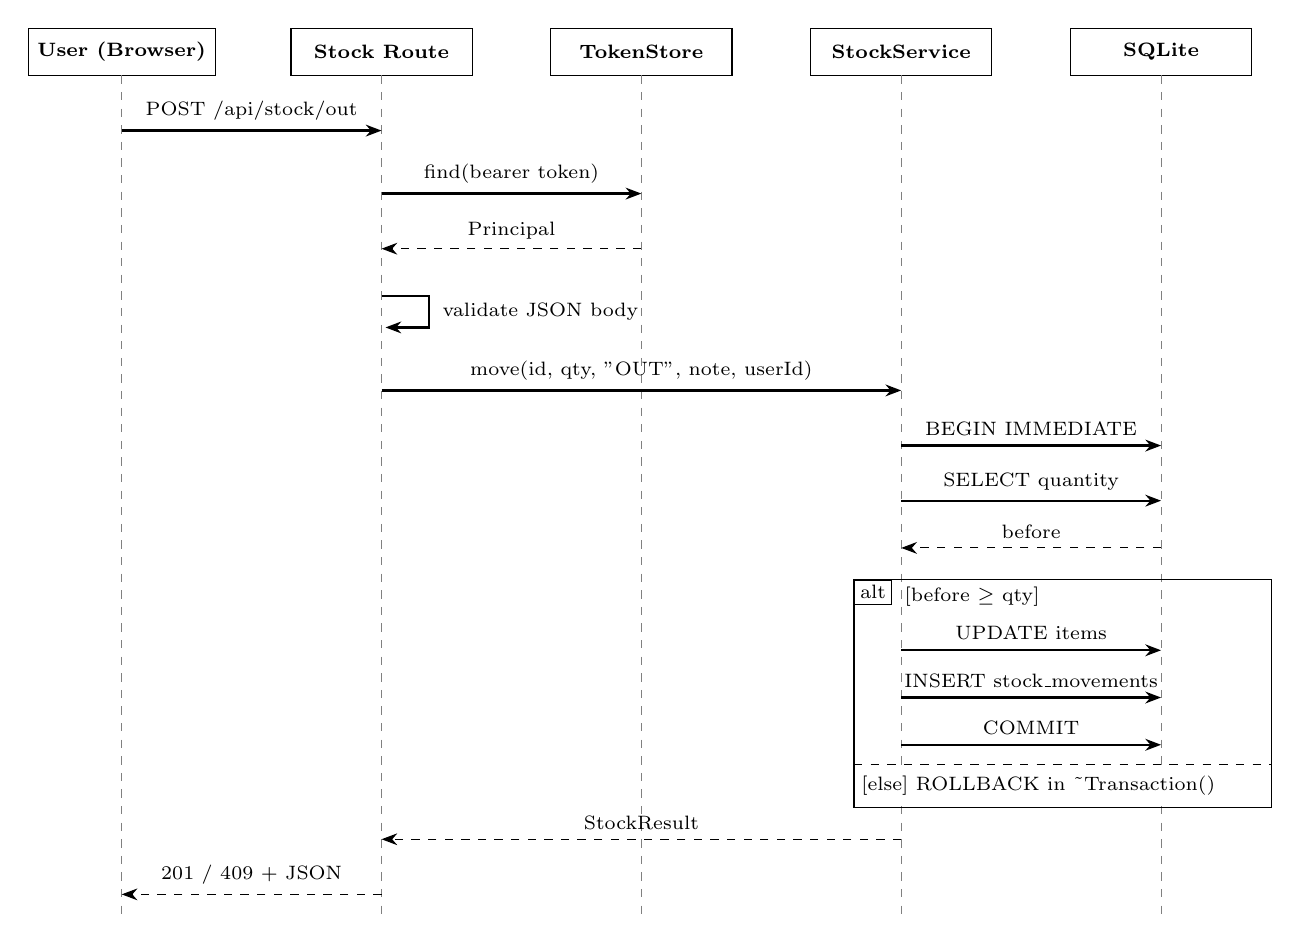
\begin{tikzpicture}[font=\scriptsize]
  \foreach \x/\n/\t in {0/u/User (Browser), 3.3/r/Stock Route, 6.6/t/TokenStore, 9.9/s/StockService, 13.2/d/SQLite} {
    \node[draw, fill=white, minimum width=2.3cm, minimum height=0.6cm, font=\scriptsize\bfseries] (\n) at (\x,0) {\t};
    \draw[dashed, gray] (\x,-0.3) -- (\x,-11.0);
  }
  \draw[msg] (0,-1.0) -- node[above]{POST /api/stock/out} (3.3,-1.0);
  \draw[msg] (3.3,-1.8) -- node[above]{find(bearer token)} (6.6,-1.8);
  \draw[ret] (6.6,-2.5) -- node[above]{Principal} (3.3,-2.5);
  \draw[msg] (3.3,-3.1) -- ++(0.6,0) -- ++(0,-0.4) -- node[above, pos=0.3]{} (3.35,-3.5);
  \node[anchor=west] at (3.95,-3.3) {validate JSON body};
  \draw[msg] (3.3,-4.3) -- node[above]{move(id, qty, "OUT", note, userId)} (9.9,-4.3);
  \draw[msg] (9.9,-5.0) -- node[above]{BEGIN IMMEDIATE} (13.2,-5.0);
  \draw[msg] (9.9,-5.7) -- node[above]{SELECT quantity} (13.2,-5.7);
  \draw[ret] (13.2,-6.3) -- node[above]{before} (9.9,-6.3);
  \draw (9.3,-6.7) rectangle (14.6,-9.6);
  \node[anchor=north west, draw, fill=white, inner sep=2pt] at (9.3,-6.7) {alt};
  \node[anchor=north west, fill=white, inner sep=1pt] at (9.9,-6.75) {[before $\ge$ qty]};
  \draw[msg] (9.9,-7.6) -- node[above]{UPDATE items} (13.2,-7.6);
  \draw[msg] (9.9,-8.2) -- node[above]{INSERT stock\_movements} (13.2,-8.2);
  \draw[msg] (9.9,-8.8) -- node[above]{COMMIT} (13.2,-8.8);
  \draw[dashed] (9.3,-9.05) -- (14.6,-9.05);
  \node[anchor=west, fill=white, inner sep=1pt] at (9.35,-9.32) {[else] ROLLBACK in \textasciitilde Transaction()};
  \draw[ret] (9.9,-10.0) -- node[above]{StockResult} (3.3,-10.0);
  \draw[ret] (3.3,-10.7) -- node[above]{201 / 409 + JSON} (0,-10.7);
\end{tikzpicture}
\end{document}
